\documentclass[12pt,letterpaper]{article}
\usepackage[margin=.7in,headheight=18pt,headsep=17pt,footskip=28pt]{geometry}
\usepackage{tikz,fancyhdr,amssymb}
\usetikzlibrary{arrows.meta}
\pdfmapfile{+cm.map}\pdfmapfile{+cmextra.map}\pdfmapfile{+symbols.map}\pdfmapfile{+latxfont.map}
\renewcommand{\familydefault}{\sfdefault}
\setlength{\parindent}{0pt}\setlength{\parskip}{9pt}
\pagestyle{fancy}\fancyhf{}
\fancyhead[L]{\small Week 66 / Lamplighter streets / Grades 3--5}
\fancyfoot[L]{\footnotesize Bellingham Math Circle / Week 66 / GGT66-S-v1}
\fancyfoot[R]{\footnotesize\thepage}\renewcommand{\headrulewidth}{.4pt}
\newcommand{\problem}[2]{\par\textbf{Problem #1:} #2\par}
\newcommand{\lineword}{\par Move word: \hrulefill\par Fewest moves: \rule{1.2in}{.4pt}\par}
% The final argument is a comma-separated list of lit lamps.
\newcommand{\street}[4]{\begin{tikzpicture}[x=#1cm,y=1cm,baseline]
\draw[line width=.8pt] (-4,0)--(4,0);
\foreach \i in {-4,...,4}{\draw[fill=white,line width=.8pt] (\i,0) circle (#2cm);\node[below=0pt,font=\small] at (\i,{-#2-.16}){\i};}
\foreach \i in {#4}{\fill (\i,0) circle (#2cm);}
\ifnum#3>-5 \fill (#3,{#2+.23})--++(-.12,.22)--++(.24,0)--cycle;\fi
\end{tikzpicture}}
\newcommand{\target}[3]{\textbf{#1}\quad\street{.63}{.12}{#2}{#3}}
\begin{document}
One move is \textbf{L}: walk left one place, \textbf{R}: walk right one place, or \textbf{F}: flip the lamp under the walker. $\circ$ is off, $\bullet$ is on, and $\blacktriangledown$ is the walker.

One partner moves the walker. The other flips the lamp, only after pointing to the walker's place. Write one letter per move. Swap jobs between targets.

\begin{center}
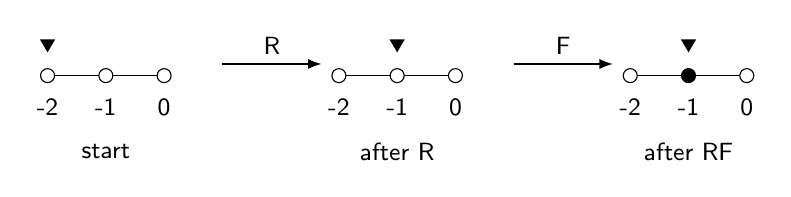
\begin{tikzpicture}[x=.74cm,y=.74cm,font=\small]
\foreach \s/\p/\lit in {0/-2/9,5/-1/9,10/-1/-1}{
\begin{scope}[shift={(\s,0)}]
\draw (-2,0)--(0,0);
\foreach \i in {-2,-1,0}{\draw[fill=white] (\i,0) circle (.12);\node[below=5pt] at (\i,0){\i};}
\ifnum\lit<2 \fill (\lit,0) circle (.12);\fi
\fill (\p,.4)--++(-.13,.22)--++(.26,0)--cycle;
\end{scope}}
\draw[-{Latex}] (1,.2)--node[above]{R}(2.7,.2);
\draw[-{Latex}] (6,.2)--node[above]{F}(7.7,.2);
\node at (-1,-1.3){start};\node at (4,-1.3){after R};\node at (9,-1.3){after RF};
\end{tikzpicture}
\end{center}
\problem{1}{Start with every lamp off and the walker at 0. Reach each target in as few moves as you can. Reset before each attempt. Use the large street for your counters.}
\begin{center}\street{1.9}{.65}{0}{}\end{center}
\target{A}{1}{1}\lineword
\target{B}{1}{-1,1}\lineword
\target{C}{0}{0,2}\lineword
\newpage
\problem{2}{Start with every lamp off and the walker at 0. These targets have the same lamps on, but the walker ends in different places. Find the fewest moves to each target.}
\begin{center}\street{1.9}{.65}{0}{}\end{center}
\vspace{.15in}
\target{A}{-2}{-2,0,2}\lineword
\vspace{.35in}
\target{B}{0}{-2,0,2}\lineword
\vspace{.35in}
\target{C}{2}{-2,0,2}\lineword
\vfill
\newpage
\problem{3}{Start with every lamp off and the walker at 0. Reach this target in the fewest moves. Find a way to convince your partner that fewer moves cannot work.}
\begin{center}\street{1.9}{.65}{0}{-1,0,1}\end{center}
\lineword
\vspace{.2in}
Workspace
\begin{center}\street{1.9}{.65}{0}{}\end{center}
\vspace{.45in}
\rule{\linewidth}{.4pt}\par\vspace{.4in}\rule{\linewidth}{.4pt}\par\vspace{.4in}\rule{\linewidth}{.4pt}\par\vspace{.4in}\rule{\linewidth}{.4pt}
\newpage
\problem{4}{Make one move from the target in Problem 3. Draw the new lamps and walker below. Find the fewest moves from \textbf{all lamps off, walker at 0} to this new target. Reset to the Problem 3 target before trying L, R, and F.}
\textbf{L}\quad\street{1.1}{.17}{-8}{}\lineword
\vspace{.2in}
\textbf{R}\quad\street{1.1}{.17}{-8}{}\lineword
\vspace{.2in}
\textbf{F}\quad\street{1.1}{.17}{-8}{}\lineword
\vspace{.2in}
\problem{5}{Can you always make a target harder to reach from all-off at 0 by making one more legal move? Use your results to settle this question.}
\vspace{.35in}\rule{\linewidth}{.4pt}\par\vspace{.35in}\rule{\linewidth}{.4pt}
\end{document}
